\documentclass[border=.1cm]{standalone}

\usepackage{tikz}
\usepackage{pgfplots}
\usepgflibrary{arrows}

\usepackage{siunitx}
\sisetup{
    detect-all = true,
    input-decimal-markers = {.},
    input-ignore = {,},
    inter-unit-product = \ensuremath{{}\cdot{}},
    multi-part-units = repeat,
    number-unit-product = \text{~},
    per-mode = fraction,
    separate-uncertainty = true,
}

\begin{document}

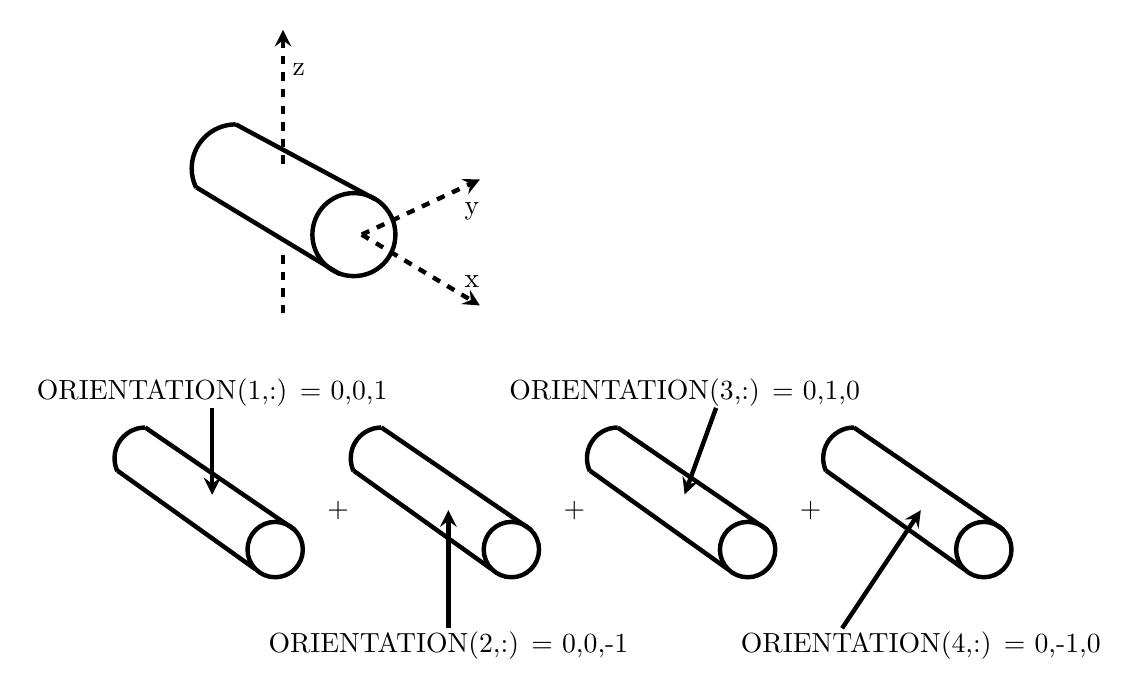
\begin{tikzpicture}

\draw [ultra thick] (0,0) circle (10pt); 
\draw[ultra thick] (-.25,-.25) -- (-2,1); 
\draw [ultra thick] (.25,.25) -- (-1.65,1.55);
\draw [ultra thick] (-1.65,1.55) arc ( 90: 205 :  .39cm);  
\draw [-stealth, ultra thick] (-.8,1.8) -- (-.8,.7); 
\node at (-.8,2) {ORIENTATION(1,:) = 0,0,1};       

\node at (.8,.5) {+};       

\draw [ultra thick] (3,0) circle (10pt); 
\draw[ultra thick] (2.75,-.25) -- (1,1); 
\draw [ultra thick] (3.25,.25) -- (1.35,1.55);
\draw [ultra thick] (1.35,1.55) arc ( 90: 205 :  .39cm);  
\draw [-stealth, ultra thick] (2.2,-1) -- (2.2,.5); 
\node at (2.2,-1.22) {ORIENTATION(2,:) = 0,0,-1};      

\node at (3.8,.5) {+};    

\draw [ultra thick] (6,0) circle (10pt); 
\draw[ultra thick] (5.75,-.25) -- (4,1); 
\draw [ultra thick] (6.25,.25) -- (4.35,1.55);
\draw [ultra thick] (4.35,1.55) arc ( 90: 205 :  .39cm);  
\draw [-stealth, ultra thick] (5.6,1.8) -- (5.2,.7); 
\node at (5.2,2) {ORIENTATION(3,:) = 0,1,0};        

\node at (6.8,.5) {+};    

\draw [ultra thick] (9,0) circle (10pt); 
\draw[ultra thick] (8.75,-.25) -- (7,1); 
\draw [ultra thick] (9.25,.25) -- (7.35,1.55);
\draw [ultra thick] (7.35,1.55) arc ( 90: 205 :  .39cm);  
\draw [-stealth, ultra thick] (7.2,-1) -- (8.2,.5); 
\node at (8.2,-1.22) {ORIENTATION(4,:) = 0,-1,0};       

\draw [ultra thick] (1,4) circle (15pt); 
\draw[ultra thick] (.82,3.5) -- (-1,4.6); 
\draw [ultra thick] (1.27,4.45) -- (-.5,5.4);
\draw [ultra thick] (-.5,5.4) arc ( 90: 206 :  .56cm);  
\draw [-stealth, ultra thick] (-.8,1.8) -- (-.8,.7);  

\draw[-stealth, dashed, ultra thick] (1.1,4) -- (2.6,3.1);  
\node at (2.5,3.4) {x};  

\draw[-stealth, dashed, ultra thick] (1.1,4) -- (2.6,4.7);  
\node at (2.5,4.3) {y};  

\draw[-stealth, dashed, ultra thick] (.1,4.9) -- (.1,6.6);   
\draw[ dashed, ultra thick] (.1,3) -- (.1,3.84);  
\node at (.3,6.1) {z}; 
 




\end{tikzpicture}

\end{document}